\subsubsection{Integration Tests}
We have seen in \autoref{integrationDia} how we chose to implement integration testing with the bottom-up approach. The way we make integration tests is by testing one connection, for instance room and monster, then add player. This means that in PlayerIntegration tests we only test the remaining connections between the player, room and monster. This way, unlike unit tests, we no longer have to test the fireball / boss connection with player and boss in the PlayerIntegration, as this is now a connection to be tested when boss gets integrated, that is, during the BossIntegration. Because of this, player now only varies on the player abilities, as room and monster are default implementations that do not get altered \todo{hvad med weather tests? Godt spørgsmål :s}. So now PlayerIntegration is fairly simple to decompose and combinate, as we only have three non-overlapping cases to look at, that is the abilities: fireball, roar and none. The structure of PlayerIntegrationTests in our repository resembles the structure of the boss. Again, we have the semantic type \textit{'playerIntegrationAbility} of a given ability, that corresponds to the combinator that contains the tests specific for that ability. Since we kept the same structure as the unit tests, the essential tests that do not vary from variation to variation is already included in the file to be combinated, meaning that if we have \textit{'playerIntegrationAbility('none)} we get a combinator with an empty string, as no tests are to be added. We can describe PlayerIntegrationTests as: \textit{string $\cap$ 'playerIntegrationAbility $\to$ MyResult $\cap$ 'playerIntegration}. \\
%\\
\begin{figure}[H]
	\centering
	\begin{tikzpicture}[grow=down, -stealth]
	%\hspace{-2cm}
	\node[bag]{Boss Integration Test} 
	child[dashed]{;\node[bag]{bossIntegrationPlayerAbility}
		child[solid]{; \node[bag]{None}}
		child[solid]{; \node[bag]{Fireball}}
	}
	child[dashed]{;\node[bag]{bossIntegrationAbility}
		child[solid]{; \node[bag]{DR}}
		child[solid]{; \node[bag]{heal}}
	};
	\end{tikzpicture}
	\caption{Taxonomy describing semantics of the boss integration tests, showcasing the simpler structure in comparison to the player unit tests.}
	\label{taxonomyBossIntegration}
\end{figure}
Now, since the connection of player and boss is tested during the BossIntegrationTests, this now looks closer to the player unit tests in the structure of the semantics. As with the playerTest, we have provided a diagram of bossIntegrationTests' taxonomy, which may help the reader easily navigate the semantic structure as discussed. This can be seen in \autoref{taxonomyBossIntegration}. In these boss integration tests, we need to take the player abilities into account, along with the boss abilities. Furthermore, because we may have a variation that does not contain the boss, we do not have boss unit tests and therefore we should neither have boss integration tests. This, just as in boss unit tests, also needs to be accounted for. However, we do not need the same intermediate step as in player unit tests, to account for the fireball boss test, as in this case, if we do not have a boss, we do not have boss integration tests at all and thus it is implied that if we do not combinate an empty boss integration file, we do indeed have a boss. As such, tests that are dependent on specific player abilities can be combinated alongside the tests specific to boss abilities as these do not overlap as they did in player unit tests. 
\begin{figure}[]
    \centering
    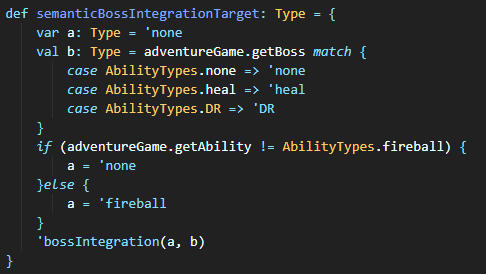
\includegraphics[width=0.6\linewidth]{Materials/TestingDiscussion/semanticBossIntegrationTarget}
    \caption{The function that specifies the boss' integration semantic targets, depending on boss abilities and player abilities.}
    \label{semanticBossIntegration}
\end{figure}
We can see in \autoref{semanticBossIntegration} the semantic target for boss integration tests. Here we can see, that like the player unit tests, we have an extra variable that depends on the player abilities. In this case, as we only have a connection between player and boss that depends on the player's fireball ability, we only have to check whether the variation includes this ability or not. However, it could easily be extended to a switch case\todo{hvad hedder det? Match case? idk} that includes the rest of the player abilities, if we made other abilities, or changed the current ones, such that other abilities than fireball had a connection with the boss and thus its integration tests. \\
Let us go over the semantics of boss integration tests. The tests specific to the player abilities, that is in our case either fireball or none, can be described as \textit{'bossIntegrationPlayerAbility}. The boss' abilities that include heal, DR and none are described as \textit{'bossIntegrationAbility}. With this in mind we can describe boss integration tests as: \textit{string $\cap$ 'bossIntegrationPlayerAbility, string $\cap$ 'bossIntegrationAbility $\to$ MyResult $\cap$ 'bossIntegration}. However, we also have the case with no boss integration tests at all, if we have any player ability, but the specific boss ability none. In this case boss can simply be described as: \textit{MyResult $\cap$ 'bossIntegration}. \\
\\
In short, the way we chose to perform integration tests, the bottom-up approach, with the classes with least dependencies at the "bottom", proved to be the right choice as this made the integration tests easier for synthesis by implementing some connections later than others, that made for simpler combinators. For instance, we can see how the boss integration test is simpler than the player unit tests, where both had to take each other into account due to the presence or abilities given, by looking at the implementations we have examined in this section. \\
We can say that integration testing was a success synthesis-wise, atleast in our case with the adventure game, as all the integration tests made for fairly simple decomposing and combinators. This means that the tests are scalable, in the case of adding more variations to the game, atleast when it comes to the boss abilities and player abilities.